\documentclass{article}
\usepackage{graphicx}
\usepackage{listings,float,wrapfig}
\usepackage[activate=true,final,tracking=true,kerning=true,spacing=true]{microtype}
\microtypecontext{spacing=nonfrench}
\usepackage[margin=2cm]{geometry}
\setlength\parindent{0pt}


\lstset{frame=tb,
language=Java,
aboveskip=3mm,
belowskip=3mm,
showstringspaces=false,
columns=flexible,
basicstyle={\small\ttfamily},
numbers=none,
numberstyle=\tiny,
  breaklines=true,
  breakatwhitespace=true,
  tabsize=3
  }
\begin{document}

\section*{Communication Protocol}
When the server is started it waits for clients to connect.

At first the server will require one client to set the lobby size, then it will allow users to login and set up their player and pawns. After this initial setup the server will enter the main game cycle and the users will be able to play the game.

The server only allows setting the lobby size once and logins with identical usernames will be forbidden, as well as logins when the lobby is full.

On client connection the server will direct the client to the lobby that is being filled. When the current lobby is full a new one will be started and successive connections will be directed to the new lobby.
A client disconnecting before logging in will be ignored, although after a client has logged in and has chosen a username its disconnection will notify the users that their lobby is being terminated.

After finishing a game either because someone won or because of an unrecoverable server error the server will notify the clients, close the lobby and clients may reconnect to play again.

After any unrecoverable error all clients are notified that the lobby will be terminated.

\vspace{8pt}

\noindent
The next sections will show in detail the communication during the different phases of a match

\subsection*{Setup: set lobby size and login}
The fist client to send a SelectPlayerNumber message containing a valid size will set the lobby to the desired size and the server will now start accepting user logins.

The users can login using an AddUser message receiving a Result specifying whether the operation completed successfully and in case it was all the users will be notified of the newly created user.

When as many users as the lobby size are added the server will send a message to the users with the gods available to choose from and it will start accepting SelectGods messages and move to the next phase.

\begin{figure}[H]
    \centering
    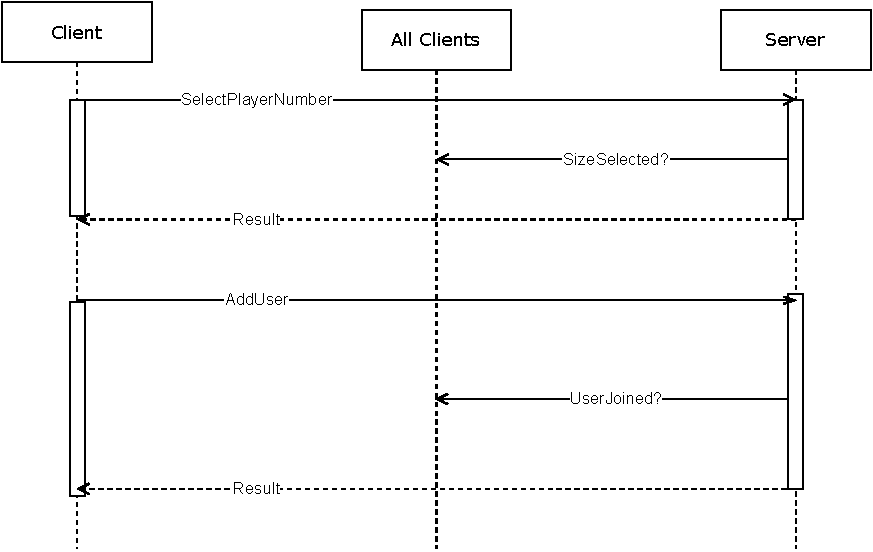
\includegraphics[width=0.85\linewidth]{communication_uml_1.pdf}
\end{figure}

\subsection*{Setup: choose divinity and place pawns}

The server will now wait for a SelectGods message, containing the list of gods, picked from the list supplied by GodsAvailable, that will be available for this game. The first user to send a valid SelectGods message will be marked as the challenger and ChooseGod requests will now be accepted from other users.

Any non-challenger user can now choose his god from the new list with a ChooseGod message, all the users will be notified of the choice with a GodChosen message and of the updated list of available gods.

After all other users have chosen their divinity the challenger will now be able to choose which user should start first with a ChooseFirstPlayer message and after that the server will start asking players to choose a starting position for their pawns.

The user will send a PlacePawn message with the desired coordinates (as with other messages the user will receive a Result and all users will be notified of successful changes).

When pawns for all users are placed the server will advance to the next phase.

\begin{figure}[H]
    \centering
    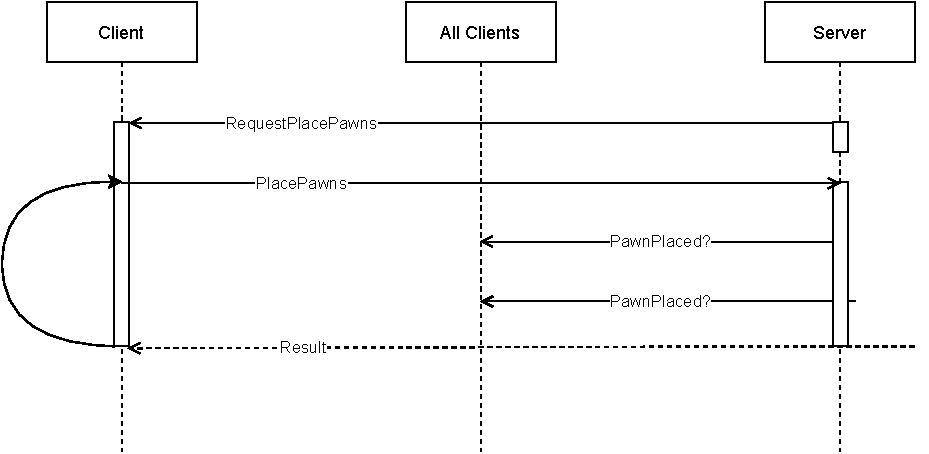
\includegraphics[width=0.85\linewidth]{communication_uml_2.pdf}
\end{figure}
\subsection*{Game cycle}

During the main game cycle the server will send ActionReady messages notifying users which user should now execute an action and which actions he is allowed to choose from. 

Users can send a CheckAction message containing the interested pawn, the desired action and the target coordinate, the server will answer with a result that will be positive if the user can execute the action with that specific pawn in that specific moment, negative otherwise. If any user other than the one previously chosen through the ActionReady message tries to execute an action it will receive a negative Result.

The user can send an ExecuteAction message that, after checking if the action is allowed, will be executed, the server will then notify all the users with the changes that happened to the model and if the move was a winning move it will send an Win message. Then, if the player's turn is not finished yet, another ActionsReady message will be sent containing the next allowed actions.

When the end of a user's turn has been reached a TurnChange message is sent and the cycle will restart asking for the next user to execute an action.

\begin{figure}[H]
    \centering
    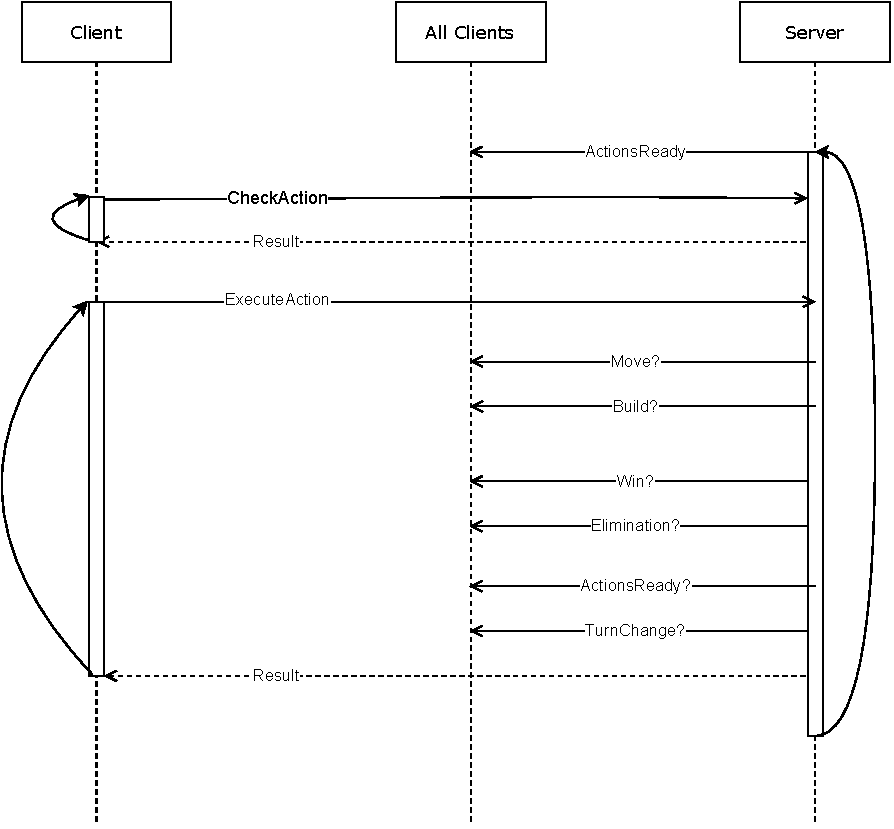
\includegraphics[width=0.85\linewidth]{communication_uml_3.pdf}
\end{figure}

\begin{wrapfigure}[6]{r}{0.46\linewidth}
    \centering
    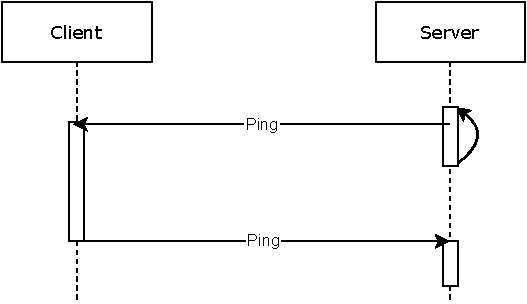
\includegraphics[width=\linewidth]{communication_uml_4.pdf}
\end{wrapfigure}

During all phases of the game the server will periodically send a PingMessage to all clients, every client must respond with a PingMessage.

If a client stops responding to pings it will be interpreted as a loss of connection, the lobby will be terminated and all users will be notified

\pagebreak
\subsection*{Message serialization}

Messages are serialized in JSON form.

\vspace{8pt}

Example message:
\begin{lstlisting}
{
    "type": "ACTION_TYPE",
    "content": {
        "user": {
            "username": "USERNAME"
        },
        "id": 0,
        "actionIdentifier": {
            "description": "MOVE"
        },
        "coordinate": {
            "x": 0,
            "y": 0
        }
    }
}
\end{lstlisting}

The \emph{type} field is used to identify the type of message through an identifier and the \emph{content} field will contain all the message specific parameters

\subsubsection*{Custom class serialization}

This section shows how the relevant non-primitive classes are serialized
\begin{lstlisting}
User:	{"username": "USERNAME"}
ActionIdentifier: {"actionIdentifier": {"description": "DESCRIPTION"}}
GodIdentifier: {"name": "NAME", "description": "DESCRIPTION"}
Coordinate: {"x": 0, "y": 0}
Building: {"level":"LEVEL0", "dome":false}
\end{lstlisting}

\subsubsection*{Messages}
Message reference
\begin{lstlisting}
    ActionsReadyMessage(User user, List<ActionIdentifier> actionIdentifiers)
    AddUserMessage(User user)
    BuildMessage(Building building, Coordinate coordinate)
    CheckActionMessage(User user, int id, ActionIdentifier actionIdentifier, Coordinate coordinate)
    ChooseFirstPlayerMessage(User self, User firstPlayer)
    ChooseGodMessage(User user, GodIdentifier god)
    EliminationMessage(User user)
    ExecuteActionMessage(User user, int id, ActionIdentifier actionIdentifier, Coordinate coordinate)
    GodChosenMessage(User user, GodIdentifier godIdentifier)
    GodsAvailableMessage(List<GodIdentifier> gods)
    MoveMessage(Coordinate from, Coordinate to)
    PawnPlacedMessage(User owner, int pawnId, Coordinate coordinate)
    PingMessage()
    PlacePawnsMessage(User user, Coordinate c1, Coordinate c2)
    RequestPlacePawnsMessage(User user)
    ResultMessage(boolean value)
    SelectGodsMessage(User user, List<GodIdentifier> gods)
    SelectPlayerNumberMessage(int size)
    ServerErrorMessage(String type, String description)
    SizeSelectedMessaege(int size)
    TurnChangeMessage(User user, int turn)
    UserJoinedMessage(User user)
    WinMessage(User user)
\end{lstlisting}
\end{document}
